\documentclass{article}

\usepackage[utf8]{inputenc}
\usepackage{amsthm}
\usepackage{amssymb}
\usepackage{mathtools}
\usepackage{graphicx}
\usepackage{mdframed}
\usepackage{float}
\usepackage[top=0.75in, bottom=0.75in, left=0.75in, right=0.75in]{geometry}
\usepackage{gauss}

\usepackage{array}
\allowdisplaybreaks

\makeatletter
\newcounter{elimination@steps}
\newcolumntype{R}[1]{>{\raggedleft\arraybackslash$}p{#1}<{$}}
\def\elimination@num@rights{}
\def\elimination@num@variables{}
\def\elimination@col@width{}
\newenvironment{elimination}[4][0]
{
    \setcounter{elimination@steps}{0}
    \def\elimination@num@rights{#1}
    \def\elimination@num@variables{#2}
    \def\elimination@col@width{#3}
    \renewcommand{\arraystretch}{#4}
    \start@align\@ne\st@rredtrue\m@ne
}
{
    \endalign
    \ignorespacesafterend
}
\newcommand{\step}[2]
{
    \ifnum\value{elimination@steps}>0\sim\quad\fi
    \left[
        \ifnum\elimination@num@rights>0
            \begin{array}
            {@{}*{\elimination@num@variables}{R{\elimination@col@width}}
            |@{}*{\elimination@num@rights}{R{\elimination@col@width}}}
        \else
            \begin{array}
            {@{}*{\elimination@num@variables}{R{\elimination@col@width}}}
        \fi
            #1
        \end{array}
    \right]
    & 
    \begin{array}{l}
        #2
    \end{array}
    \addtocounter{elimination@steps}{1}
}
\makeatother

\DeclarePairedDelimiter{\abs}{\lvert}{\rvert}
\DeclarePairedDelimiter{\norm}{\lvert \lvert}{\rvert \rvert}

\newtheoremstyle{break}% name
  {}%         Space above, empty = `usual value'
  {}%         Space below
  {\itshape}% Body font
  {}%         Indent amount (empty = no indent, \parindent = para indent)
  {\bfseries}% Thm head font
  {.}%        Punctuation after thm head
  {\newline}% Space after thm head: \newline = linebreak
  {}%         Thm head spec

\newtheorem{Def}{Definition}[section]

\theoremstyle{break}

\newtheorem{innerEx}{Exempel}[section]
\newtheorem{sats}{Sats}[section]
\newtheorem{Rem}{Anmärkning}[]

\newenvironment{Ex}
{\begin{mdframed} \begin{innerEx} \vspace{3pt}}
{\vspace{3pt} \end{innerEx} \end{mdframed}}  

\newenvironment{bevis}
{\begin{mdframed} \begin{proof} \vspace{3pt}}
{\vspace{3pt} \end{proof} \end{mdframed}}


\title{
	 Linjär Algebra\\
	 Föreläsning 11
    \author{Erik Sjöström}
}
\begin{document}
\maketitle
\section{Räkneexempel} % (fold)
\label{sec:r_kneexempel}
Antag att vi har en 2D-platta vars kanttemperatur hålls konstant. Vi vill veta temperaturen i det inre av plattan.
\begin{center}
	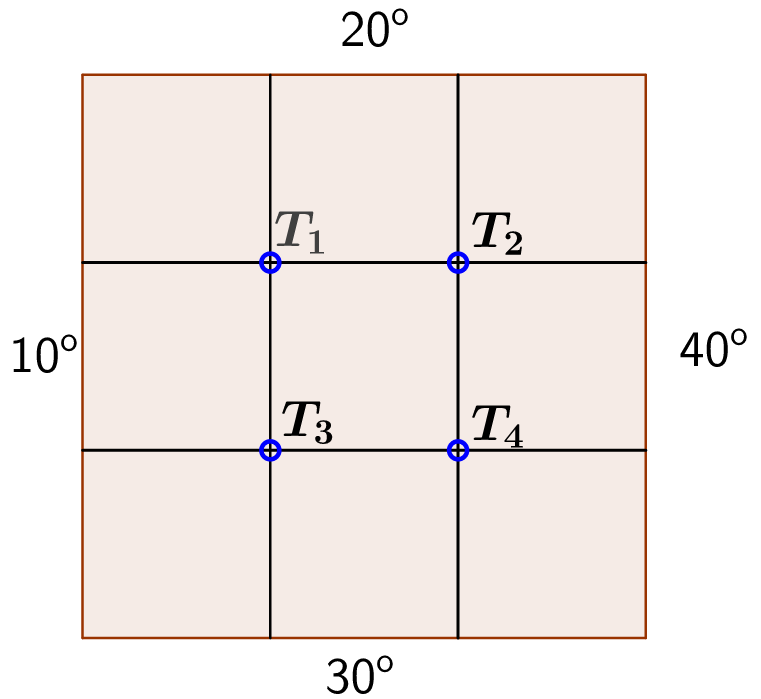
\includegraphics[scale=0.25]{platta.png}
\end{center}
Temperaturen kan approximeras med följande medelvärden:
\begin{gather*}
	T_1 = \frac{10 + 20 + T_2 + T_3}{4} \Leftrightarrow 4T_1 - T_2 - T_3 = 30\\
	T_2 = \frac{T_1 + 20 + 40 + T_4}{4} \Leftrightarrow 4T_2 - T_1 - T_4 = 60\\
	T_3 = \frac{10 + T_1 + T_4 + 30}{4} \Leftrightarrow 4T_3 - T_1 - T_4 = 40\\
	T_4 = \frac{T_3 + T_2 + 40 + 30}{3} \Leftrightarrow 4T_4 - T_3 - T_2 = 70
\end{gather*}
\[
    \begin{cases}
    	4T_1 - T_2 - T_3 = 30\\
    	-T_1 + 4T_2 - T_4 = 60\\
    	-T_1 + 4T_3 - T_4 = 40 \\
    	-T_2 -T_3 + 4T_4 = 70
    \end{cases}
\]
Dvs:
\[
    \begin{bmatrix} 
    4 & -1 & -1 & 0\\
    -1 & 4 & 0 & -1\\
    -1 & 0 & 4 & -1\\
    0 & -1 & -1 & 4\\
    \end{bmatrix}
    \cdot \begin{bmatrix} T_1\\T_2\\T_3\\T_4 \end{bmatrix} = \begin{bmatrix} 30\\60\\40\\70 \end{bmatrix}
\]
Som har totalmatris:
\begin{elimination}[1]{4}{1.75em}{1.1}
\step
{
	4 & -1 & -1 & 0 & 30\\
    -1 & 4 & 0 & -1 & 60\\
    -1 & 0 & 4 & -1 & 40\\
    0 & -1 & -1 & 4 & 70\\
}
{
	\\
	\\
	\\
	\\
}
\end{elimination}
Som vi kan gausseliminera till trappstegsform, så att alla rader har fler inledande nollor än raden ovanför.
Svaret blir: (i reducerad trappstegsform)
\begin{elimination}[1]{4}{2em}{1.1}
\step
{
	1 & 0 & 0 & 0 & 20.0\\
	0 & 1 & 0 & 0 & 27.5\\
	0 & 0 & 1 & 0 & 22.5\\
	0 & 0 & 0 & 1 & 30.0\\
}
{
	\\
	\\
	\\
	\\
}
\end{elimination}
\begin{Rem}
    Programmvara t.ex. "rref" i Matlab svarar i reducerad trappstegsform.
\end{Rem}
% section r_kneexempel (end)
\section{Elementärmatris} % (fold)
\label{sec:element_rmatris}
Man kan uttrycka gausseliminering som en matrismultiplikation.
\begin{Def}
    En elementärmatris \textbf{E} är en matris som erhålls genom att utföra \underline{en} elementär radoperation på \textbf{I}.
\end{Def}
\begin{Rem}
    \[
        \mathbf{I} = \begin{bmatrix}
        1 & 0 & \cdots & 0\\
        0 & 1 & \cdots & 0\\
        \vdots & \vdots & \ddots & \vdots\\
        0 & 0 & \cdots & 1
         \end{bmatrix}
    \]
\end{Rem}
\noindent
De elementära radoperationerna är:
\begin{itemize}
	\item Addition: Addera till en rad en multipel av en annan rad
	\item Platsbyte: Låt två rader byta plats
	\item Skalning: Multiplicera en rad med en konstant $\neq 0$
\end{itemize}
Om \textbf{E} är en ($m \times n$) elementärmatris och \textbf{A} är en ($m \times n$)-matris. Så är $\mathbf{E} \cdot \mathbf{A}$ den ($m \times n$)-matris som man får genom att på \textbf{A} utföra den radoperation som gjordes på \textbf{I} för att ge \textbf{E}.
\begin{Ex}
    Låt:
    \begin{align*}
    &&\mathbf{A} = \begin{bmatrix} 2 & 5\\-3&-7 \end{bmatrix}
    &&\mathbf{E}_1 = \overbrace{\begin{bmatrix} 1 & 0\\3/2 & 1 \end{bmatrix}}^{\frac{3}{2} \cdot R_1 \cdot R_2}
    \end{align*}
    \[
        \mathbf{E}_1 \cdot \mathbf{A} = \begin{bmatrix} 1 & 0\\3/2 & 1 \end{bmatrix} \cdot \begin{bmatrix} 2&5\\-3&-7 \end{bmatrix} = \begin{bmatrix} 2&5\\0&1/2 \end{bmatrix}
    \]
    Om vi nu bildar tre elementärmatriser till:
    \begin{align*}
    &&\mathbf{E}_2 = \overbrace{\begin{bmatrix} 1&0\\0&2 \end{bmatrix}}^\text{$R_2 \cdot 2$}
    &&\mathbf{E}_3 = \overbrace{\begin{bmatrix} 1&-5\\0&1 \end{bmatrix}}^\text{$-5 \cdot R_2 + R_1$}
    &&\mathbf{E}_4 = \overbrace{\begin{bmatrix} 1/2&0\\0&1 \end{bmatrix}}^\text{$\frac{1}{2} \cdot R_1$}
    \end{align*}
    Så kan vi bilda matrisen:
    \[
        \mathbf{E}_4 \cdot \mathbf{E}_3 \cdot \mathbf{E}_2 \cdot \mathbf{E}_1 \cdot \mathbf{A} = \begin{bmatrix} 1/2&0\\0&1 \end{bmatrix} \cdot \begin{bmatrix} 1&-5\\0&1 \end{bmatrix} \cdot \begin{bmatrix} 1&0\\0&2 \end{bmatrix} \cdot \begin{bmatrix} 1 & 0\\3/2 & 1 \end{bmatrix} \cdot \begin{bmatrix} 2&5\\-3&-7 \end{bmatrix} = ... = \mathbf{I}
    \]
\end{Ex}
\begin{Rem}
    Detta används mest i bevis-sammanhang
\end{Rem}
% section element_rmatris (end)
\section{Inverterbarhet} % (fold)
\label{sec:inverterbarhet}
Elementärmatrisen \textbf{E} är inverterbar.
\[
    \mathbf{E} \cdot \mathbf{E}^{-1} = \mathbf{E}^{-1} \cdot \mathbf{E} = \mathbf{I}
\]
Inversen av \textbf{E} kan tolkas som:
\begin{center}
	"Hur får jag radoperationen i \textbf{E} ogjord?"
\end{center}
\begin{Ex}
    \[
        \mathbf{E}_1^{-1} \cdot \mathbf{E}_1 \cdot A = \overbrace{\begin{bmatrix} 1&0\\-3/2&1 \end{bmatrix}}^{R_2 - \frac{3}{2} \cdot R_1} \cdot \overbrace{\begin{bmatrix} 1&0\\3/2&1 \end{bmatrix}}^{R_2 + \frac{3}{2} \cdot R_1}\cdot \begin{bmatrix} 2&5\\-3&-7 \end{bmatrix} = \begin{bmatrix} 2&5\\-3&-7 \end{bmatrix} = \mathbf{A}
    \]
\end{Ex}
\begin{sats}
    Om två matriser \textbf{A}, \textbf{B} är inverterbara så är produkten $\mathbf{A} \cdot \mathbf{B}$ också inverterbar, och:
    \[
        (\mathbf{A} \cdot \mathbf{B})^{-1} = \mathbf{B}^{-1} \cdot \mathbf{A}^{-1}
    \]
\end{sats}
\begin{sats}
    Produkten av flera inverterbara matriser är inverterbara.
\end{sats}
\begin{sats}
    Låt \textbf{A} vara en ($n \times m$)-matris. Följande utsagor är ekvivalenta:
    \begin{enumerate}
    	\item $\mathbf{A} \cdot \vec{x} = \vec{b}$ har en unik lösning för alla $\vec{b}$.
    	\item Varje reduktion av \textbf{A} till trappstegsform saknar fria kolumner.
    	\item Man kan reducera \textbf{A} till \textbf{I} med hjälp av elementära radoperationer.
    	\item Matrisen \textbf{A} är inverterbar.
    \end{enumerate}
\end{sats}
Så om vi finner att en utsaga gäller, så vet vi att lla andra också gäller, och vice versa.
\paragraph{Bevisresonemang:} % (fold)
\label{par:bevisresonemang}
Antag att (4) gäller, dvs \textbf{A} inverterbar.\\
Betrakta:
\[
    \mathbf{A} \cdot \vec{x} = \vec{b} \Leftrightarrow \mathbf{A}^{-1} \cdot \mathbf{A} \cdot \vec{x} = \mathbf{A}^{-1} \cdot \vec{b} \Leftrightarrow \vec{x} = \mathbf{A}^{-1} \cdot \vec{b}
\]
Eftersom $\mathbf{A}^{-1}$ är unik så är $\mathbf{A}^{-1} \cdot \vec{b}$ unik.\\
Dvs:
\[
    (4) \Rightarrow (1)
\]
Antag att (1) gäller, dvs $\mathbf{A} \cdot \vec{x} = \vec{b}$ har en unik lösning.\\
Vi har löst $\mathbf{A} \cdot \vec{x} = \vec{b}$ genom gausseliminering av:
\[
    \begin{bmatrix} 
    \begin{array}{c|c}
    	\mathbf{A} & \vec{b}
    \end{array}
    \end{bmatrix}
\]
och fått:
\[
    \begin{bmatrix} 
    \begin{array}{c|c}
    	\mathbf{u} & \vec{d}
    \end{array}
    \end{bmatrix}
\]
\begin{Rem}
    Kom ihåg satsen från F10:
    \begin{mdframed}    
    \begin{center}
    	\begin{sats}
    Antag att totalmatrisen
    $\begin{bmatrix}
    \begin{array}{c|c}
        \mathbf{A}& \vec{b}
    \end{array}
    \end{bmatrix}$
     gauselimineras med elementära radoperationer till en reducerad trappstegsform och kallar den för
     $\begin{bmatrix}
    \begin{array}{c|c}
        \mathbf{u}& \vec{d}
    \end{array}
    \end{bmatrix}$
    . Då gäller:
    \begin{itemize}
        \item Om sista kolumnen i $\begin{bmatrix}
    \begin{array}{c|c}
        \mathbf{u}& \vec{d}
    \end{array}
    \end{bmatrix}$ är en pivotkolumn saknar systemet lösningar. (dvs: $\vec{d}$ är en pivotkolumn)
    \item Om sista kolumnen i $\begin{bmatrix}
    \begin{array}{c|c}
        \mathbf{u}& \vec{d}
    \end{array}
    \end{bmatrix}$ inte är en pivotkolumn och antalet pivotkolumner är färre än antalet variabler så finns det oändligt många lösningar.
    \item Om alla kolumner i \textbf{u} är pivotkolumner så finns det exakt en lösning.
    \end{itemize}
\end{sats}
    \end{center}
    \end{mdframed}
\end{Rem}
\noindent
Eftersom $\mathbf{A} \cdot \vec{x} = \vec{b}$ har en unik lösning gäller det att alla kolumner i \textbf{u} är pivotkolumner. (inga fria kolumner)\\
Dvs:
\[
    (1) \Rightarrow (2)
\]
Antag att vi reducerat \textbf{A} till trappstegsform:
\begin{itemize}
	\item Man kan få 1:or på diagonalen.
	\item Vi kan nollställa alla element ovanför med elementära radoperationer.
\end{itemize}
Man kan alltså reducera \textbf{A} till \textbf{I} med elementära radoperationer.\\
Dvs:
\[
    (1) \Rightarrow (3)
\]
Antag (2) dvs varje reduktion av \textbf{A} saknar fria kolumner:
\begin{elimination}[1]{1}{1.75em}{1.1}
\step
{
	\textbf{A} & \vec{b}
}
{
	\\
}
\step
{
	\textbf{u} & \vec{d}
}
{
	\\
}
\end{elimination}
Men $\mathbf{A}_{n \times n}$ dvs $\mathbf{u}_{n \times n}$. Vi har ett pivotelement i varje rad i \textbf{u}, dvs det finns inget pivotelement i $\vec{d}$.\\
Dvs: det finns exakt en lösning
\[
    (2) \Rightarrow (1)
\]
% paragraph bevisresonemang (end)
\begin{bevis}
	Antag (3) (visa $\Rightarrow$ inverterbar)\\
	Eftersom \textbf{A} kan gausselimineras till \textbf{I} så finns det
	\[
	    \mathbf{E}_1, \mathbf{E}_2, ..., \mathbf{E}_k
	\]
	elementära matriser sådana att:
	\[
	    \overbrace{\mathbf{E}_k \cdot \mathbf{E}_{k-1} \cdot ... \cdot \mathbf{E}_2 \cdot \mathbf{E}_1}^{\mathbf{B}} \cdot \mathbf{A} = \mathbf{I}
	\]
	$\mathbf{E}_1, \mathbf{E}_2, ..., \mathbf{E}_k$ är inverterbara och därmed även produkten \textbf{B}.\\
	Eftersom $\mathbf{B} \cdot \mathbf{A} = \mathbf{I}$ så måste $\mathbf{B}^{-1} = \mathbf{A}$.\\
	Dvs: \textbf{A} inverterbar och $\mathbf{A}^{-1} = \mathbf{B}$.
\end{bevis}
\begin{Rem}
    Detta bevis ger oss ett sätt att bestämma inversen för \textbf{A}. Nämligen:
    \begin{itemize}
    	\item Bilda:
    	\begin{elimination}[1]{1}{1.75em}{1.1}
		\step
		{
			\textbf{A} & \textbf{I}
		}
		{
			\\
		}
		\step
		{
			\textbf{I} & \textbf{u}
		}
		{
			\\
		}
		\end{elimination}
		\item Om $\mathbf{A}^{-1}$ finns så är $\mathbf{u} = \mathbf{A}^{-1}$
    \end{itemize}
\end{Rem}
\newpage
\begin{Ex}
    Bestäm $\mathbf{A}^{-1}$ om:
    \[
        \mathbf{A} = \begin{bmatrix} 2&5\\-3&-7 \end{bmatrix}
    \]
    \begin{elimination}[2]{2}{1.75em}{1.1}
    \step
    {
    2 & 5 & 1 & 0\\
    -3 & -7 & 0 & 1\\
    }
    {
    \\
    + R_1 \cdot \frac{3}{2}
    }
    \step
    {
    2 & 5 & 1 & 0\\
    0 & \frac{1}{2} & \frac{3}{2} & 1
    }
    {
    + R_1 \cdot -10\\
    \\
    }
    \end{elimination}
    \begin{elimination}[2]{2}{1.75em}{1.1}
    \step
    {
    2 & 0 & -14 & -10\\
    0 & \frac{1}{2} & \frac{3}{2} & 1\\
    }
    {
    \cdot \frac{1}{2}\\
    \cdot 2\\
    }
    \step
    {
    1 & 0 & -7 & -5\\
    0 & 1 & 3 & 2\\
    }
    {
    \\
    \\
    }
    \end{elimination}
    Så vi får att:
    \[
        \mathbf{A}^{-1} = \begin{bmatrix} -7&-5\\3&2 \end{bmatrix}
    \]
\end{Ex}

% section inverterbarhet (end)



\end{document}